\section{Verbale della riunione}

	\subsection{Cruscotto - Google Sheet}
	Dalle varie informazioni e dati presenti in Google Sheet, il gruppo ha deciso di inserire nel \textsc{Piano di Qualifica} le metriche inserite nel file al link  \url{https://threewaymilkshake.atlassian.net/wiki/spaces/VER/pages/158924809/2021-02-10+VI-10} .
\\	E` stata pensata inoltre una metrica relativa all'uniformità di lavoro nel tempo del gruppo. Questa metrica potrebbe non essere utile in quanto siamo studenti e non lavoratori che possono concentrarsi solo sul lavoro. Si valuterà se utilizzarla verso la fine della RP.\\
Per e metriche che darebbero valori fissi si è deciso di:
\begin{itemize}
	\item Ottenere misurazioni periodiche per mostrare a fine periodo l'andamento di tali indici;
	\item se sono abbastanza, ognuno sarà incaricato di effettuare una "fotografia" periodica delle metriche.
\end{itemize}
\begin{center}
	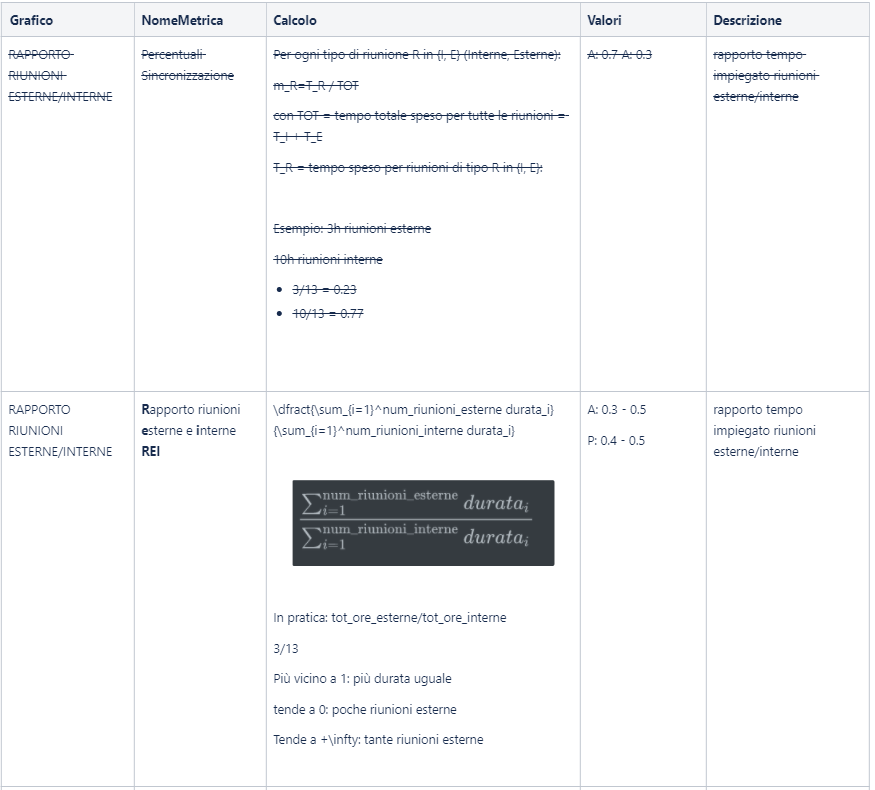
\includegraphics[scale=0.8]{g1}\\
	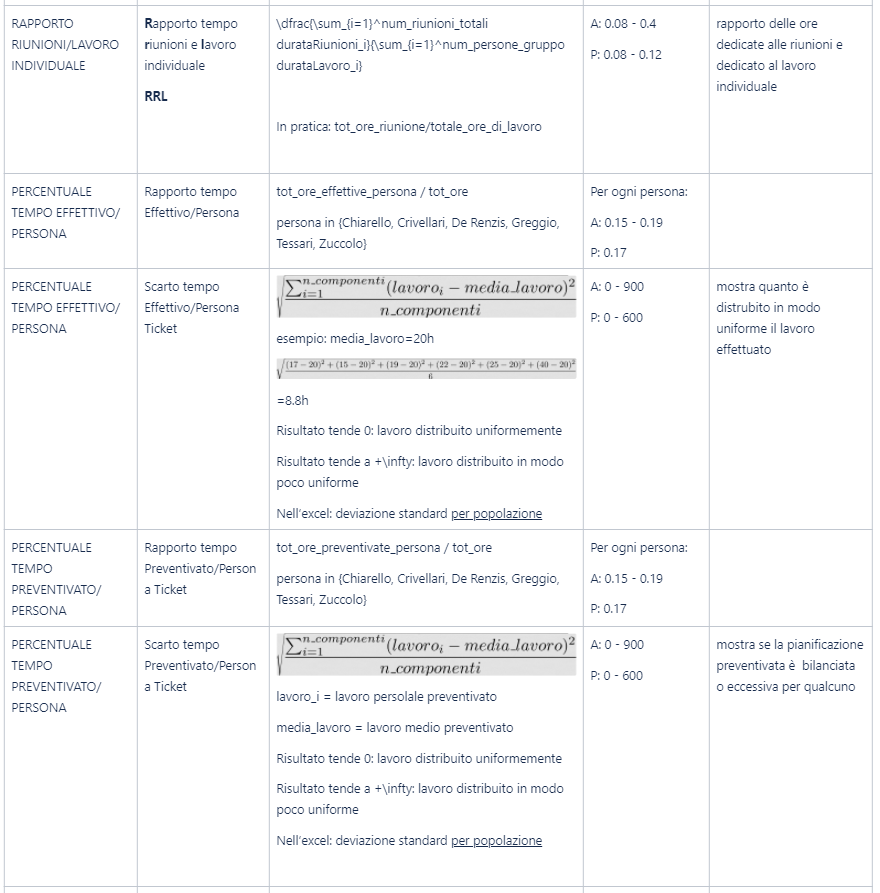
\includegraphics[scale=0.8]{g2}\\
	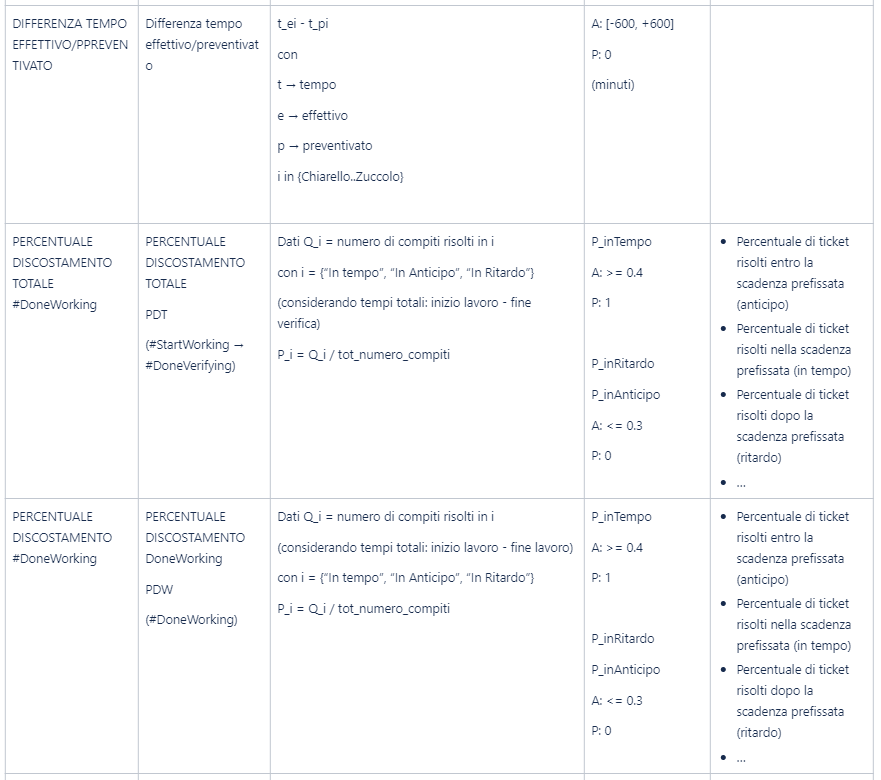
\includegraphics[scale=0.8]{g3}\\
	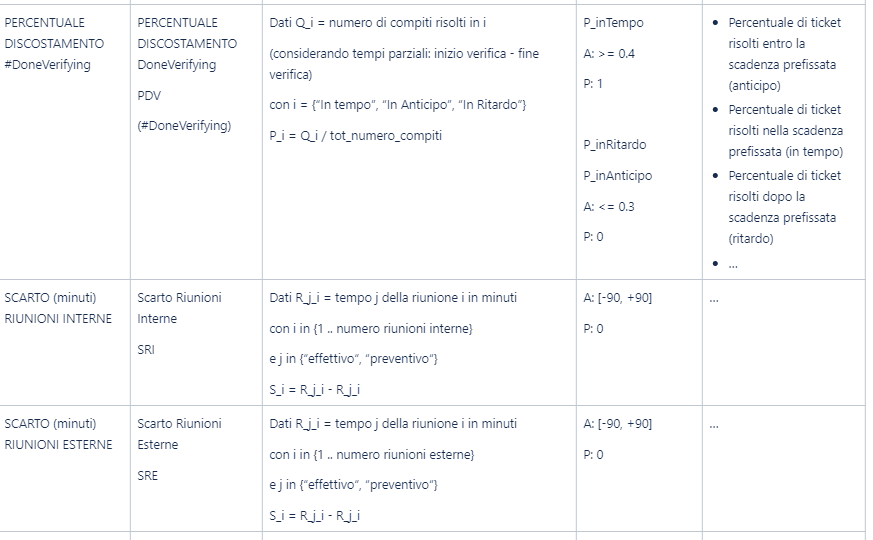
\includegraphics[scale=0.8]{g4}\\
\end{center}

	
	\subsection{Aggiunte al workflow}
	\subsubsection{Inizio nuova task}
	\begin{enumerate}
		\item Si prende il codice della task da Jira: PCS-\#\#\# e si va sull’Excel \textbf{Sincronizzazione Dati} nella riga corrispondente \textbf{TEMPO (minuti) PREVENTIVATO} → tempo durata preventivato (relativo al lavoro);
		\item in \textbf{ATA \#StartWorking → \#DoneWorking: }
		\begin{itemize}
			\item Settare date: \textbf{AVVIO} e \textbf{SCADENZA PREFISSATA};
			\item Ogni qualvolta si committa con 'git commit -m “PCS-\#\#\# \#comment <commento> \#time <tempo>” ' (quindi usando tracciamento temporale di Jira) e si incrementa sull’excel.
		\end{itemize}
	\item Al termine del lavoro della task si dovrà andare ad inserire la data di fine effettiva della colonna \textbf{DATA \#StartWorking → \#DoneWorking FINE EFFETTIVA};
	\item Aggiungere il \textbf{TEMPO (minuti) EFFETTIVO} con relativo \textbf{Ruolo};
	\item quando finito controllare; \url{https://threewaymilkshake.atlassian.net/wiki/spaces/VER/pages/138412040/Sequenza+Stesura+e+Verifica+verbali} e assegnare la verifica a chi tocca, secondo l’ordine.
	\end{enumerate}

	\subsubsection{Verifica task}
	\begin{enumerate}
		\item Si prende il codice della task da Jira: PCS-\#\#\# e si va sull’Excel \textbf{Sincronizzazione Dati} nella riga corrispondente \textbf{TEMPO (minuti) PREVENTIVATO} → tempo durata preventivato (relativo alla verifica);
		\item settare \textbf{SCADENZA PREFISSATA} in \textbf{DATA \#StartVerifying → \#DoneVerifying};
		\item Al termine della verifica si dovrà andare ad inserire la data di fine effettiva della colonna \textbf{DATA \#StartVerifying → \#DoneVerifying AVVIO (=EFFETTIVA FINE DI \#TOVERIFY) FINE EFFETTIVA}.
		
	\end{enumerate}

	\subsubsection{Riunione}
	Chi dovrà redigere il verbale dovrà::
	\begin{enumerate}
		\item In \textbf{Durata Riunioni - Dati} inserire la \textbf{Data, Prevista ed Effettiva}  sotto \textbf{Durata riunioni interne / esterne};
		\item Creare branch feature/VT-n con T → {I, E}, n → numero
		\item Quando finito, oltre a settare tempi come per task normali, controllare file in \url{https://threewaymilkshake.atlassian.net/wiki/spaces/VER/pages/138412040/Sequenza+Stesura+e+Verifica+verb} e:
		\begin{itemize}
			\item Checkare la propria box;
			\item Una volta che la task è in toVerify con l’assignee cancellato (si cancella da solo tramite automazione) assegnare a chi tocca la verifica.
		\end{itemize}
		\item Spostare note su Confluence → Trascritti.
	\end{enumerate}

	\subsection{Stesura verbali}
	Si è deciso di avere al massimo 3 giorni di tempo per la stesura dei verbali e massimo 2 giorni di tempo per la loro verifica.
	
	\subsection{Verifica}
	Si è deciso che ognuno dovrà impostare l'assegnatario del processo di verifica una volta svolto la propria task secondo la tabella contenuta in \url{https://threewaymilkshake.atlassian.net/wiki/spaces/VER/pages/138412040/Sequenza+Stesura+e+Verifica+verb}.
	\begin{center}
		\item 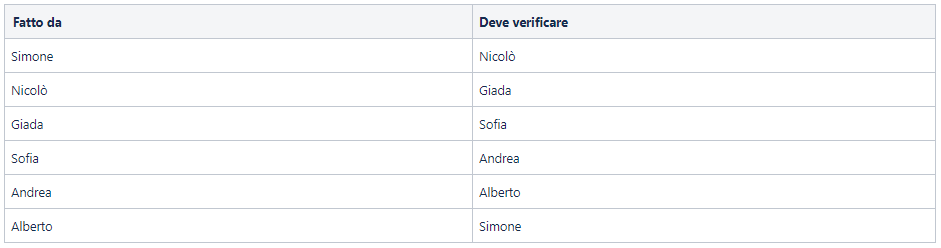
\includegraphics[scale=0.8]{tabella}\\
	\end{center}

	\subsection{Incontri con i docenti}
	Si è scelto di non creare verbali per gli incontri con i docenti.\\
	Verranno comunque presi appunti sui vari meeting con i professori in un documento privato del gruppo su Confluence.

	